% !TEX encoding = UTF-8 Unicode
%!TEX TS-program = xelatex

\documentclass[12pt]{extarticle}
% extarticle is like article but can handle 8pt, 9pt, 10pt, 11pt, 12pt, 14pt, 17pt, and 20pt text

\def \ititle {Origins of Mind}
 
\def \isubtitle {Lecture 08}
 
\def \iauthor {Stephen A. Butterfill}
\def \iemail{s.butterfill@warwick.ac.uk}
\date{}

%for strikethrough
\usepackage[normalem]{ulem}

\input{$HOME/Documents/submissions/preamble_steve_handout}

%logic symbol \leftmodels
\usepackage{MnSymbol}

%\bibpunct{}{}{,}{s}{}{,}  %use superscript TICS style bib
%remove hanging indent for TICS style bib
%TODO doesnt work
\setlength{\bibhang}{0em}
%\setlength{\bibsep}{0.5em}


%itemize bullet should be dash
\renewcommand{\labelitemi}{$-$}

\begin{document}

%\raggedcolumns

\begin{multicols*}{3}

\setlength\footnotesep{1em}


\bibliographystyle{newapa} %apalike

%\maketitle
%\tableofcontents




%--------------- 
%--- start paste

\def \ititle {Logic I}
 
\def \isubtitle {Lecture 06}
 
\begin{center}
 
{\Large
 
\textbf{\ititle}: \isubtitle
 
}
 
 
 
\iemail %
 
\end{center}
 
Readings refer to sections of the course textbook, \emph{Language, Proof and Logic}.
 
 
 
\section{∨Intro and ∨Elim}
 
\emph{Reading:} §6.2
 
\begin{center}
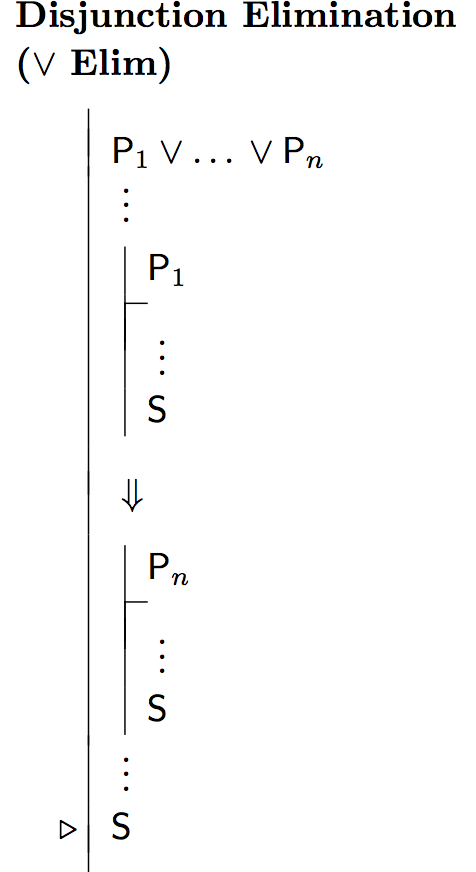
\includegraphics[scale=0.3]{img/rule_disjunction_elim.png}
\end{center}
\begin{center}
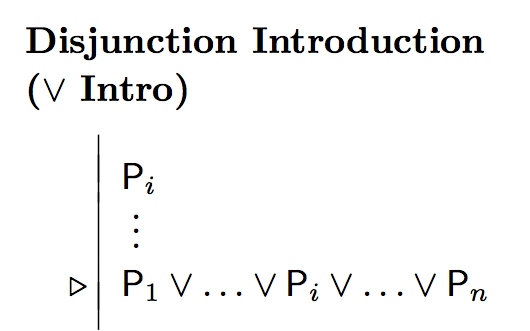
\includegraphics[scale=0.3]{img/rule_disjunction_intro.png}
\end{center}
 
 
\section{∨Elim and Soundness}
 
\emph{Reading:} §5.2, §6.2
 
 
 
\section{∨Elim: An Example}
 
To prove a conclusion from a disjunction, prove it from each disjunct.
 
\begin{center}
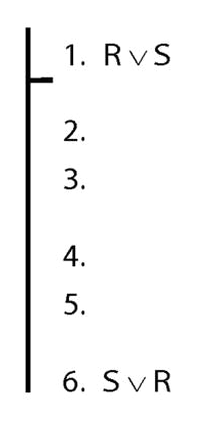
\includegraphics[scale=0.3]{img/proof_disjunction_elim.png}
\end{center}


\vfill
\columnbreak
 
 
\section{Not Or}
 
\emph{Reading:} §3.7
 
\begin{center}
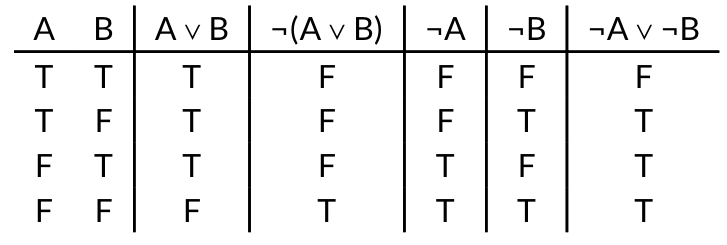
\includegraphics[scale=0.3]{img/tt_unit_603.png}
\end{center}
 
 
\section{→Intro: An Example}
 
\begin{center}
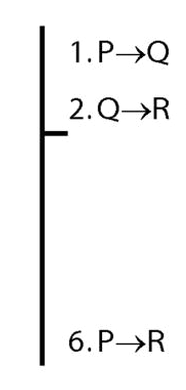
\includegraphics[scale=0.3]{img/proof_arrow_intro.png}
\end{center}
 
 
\section{¬Elim}
 
\emph{Reading:} §6.3
 
\begin{center}
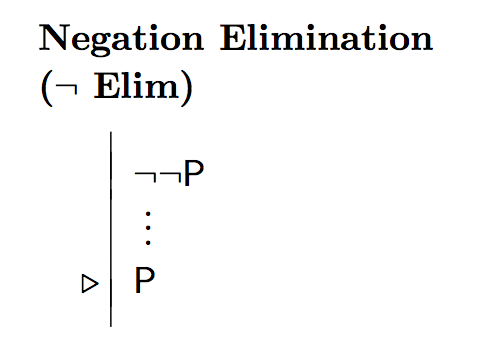
\includegraphics[scale=0.3]{img/rule_negation_elim.png}
\end{center}
 
 
\section{¬Intro}
 
\emph{Reading:} §5.3, §6.3
 
\begin{center}
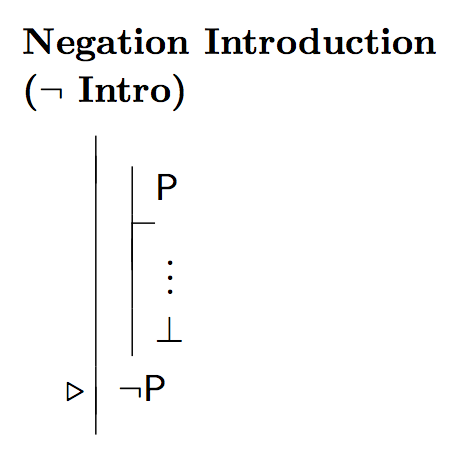
\includegraphics[scale=0.3]{img/rule_negation_intro.png}
\end{center}
\begin{center}
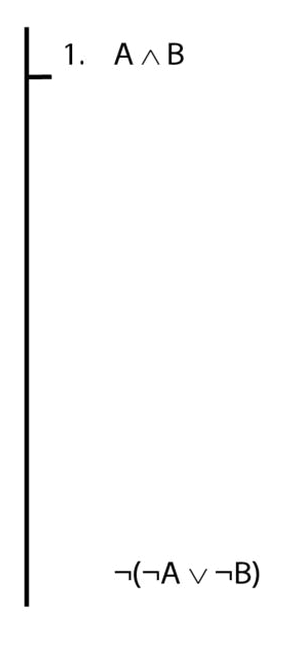
\includegraphics[scale=0.3]{img/proof_example_unit_281.png}
\end{center}

\vfill
\columnbreak
 
\section{Subproofs Are Tricky}
 
What is wrong with the following apparent proof?
 
\begin{center}
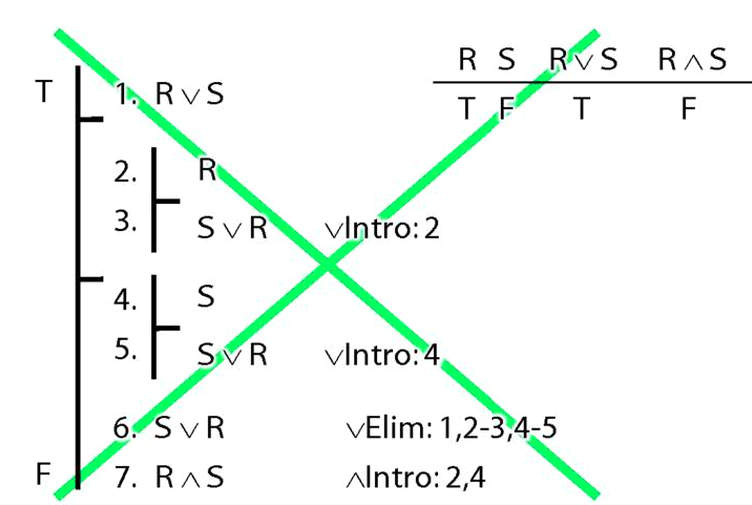
\includegraphics[scale=0.3]{img/unit_224_subproofs_tricky.png}
\end{center}

%--- end paste
%--------------- 
 


\end{multicols*}

\end{document}